% Shared preamble of the FFNOML documents (docs/physics/ffno-physics.tex, docs/technical/ffno-technical.tex).
\documentclass[10pt]{extarticle}
\usepackage[a4paper,margin=2cm]{geometry}
\usepackage[T1]{fontenc}\usepackage{lmodern}\usepackage{tabularx}
\usepackage{amsmath,amssymb,bm,enumitem,titlesec,xcolor,booktabs,array,graphicx,longtable,listings,float,caption}
\usepackage{tikz}\usetikzlibrary{arrows.meta,positioning,calc,fit,shapes.geometric}
\PassOptionsToPackage{obeyspaces,spaces}{url}
\usepackage{xurl}
\usepackage[hidelinks]{hyperref}
\urlstyle{tt}
\definecolor{ink}{HTML}{1F3A5F}\definecolor{boxa}{HTML}{E8F0FA}\definecolor{boxb}{HTML}{FCEFE6}\definecolor{boxc}{HTML}{E9F6F0}\definecolor{boxd}{HTML}{F3F1FB}
\titleformat{\section}{\large\bfseries\color{ink}}{\thesection.}{0.5em}{}
\titlespacing*{\section}{0pt}{12pt}{4pt}
\titleformat{\subsection}{\normalsize\bfseries}{\thesubsection}{0.5em}{}
\titlespacing*{\subsection}{0pt}{8pt}{2pt}
\titleformat{\subsubsection}{\normalsize\itshape}{\thesubsubsection}{0.5em}{}
\setlist{nosep,leftmargin=1.4em}
\setlength{\parindent}{0pt}\setlength{\parskip}{5pt}
\renewcommand{\arraystretch}{1.15}
\captionsetup{font=small,labelfont=bf,skip=4pt}
\newcommand{\code}[1]{\nolinkurl{#1}}
\newcommand{\dd}{\mathrm{d}}
\newcommand{\nel}{n_{\rm e}}
\newcommand{\vlos}{v_{\rm los}}
\newcommand{\vturb}{v_{\rm turb}}
\newcommand{\Halpha}{H$\alpha$}
\newcolumntype{L}[1]{>{\raggedright\arraybackslash}p{#1}}
\newcolumntype{Y}{>{\raggedright\arraybackslash}X}
\newcommand{\doctitle}[2]{{\LARGE\bfseries\color{ink} #1}\\[4pt]{\small #2}\par\vspace{4pt}}
\lstset{basicstyle=\ttfamily\footnotesize,breaklines=true,columns=fullflexible,frame=single,rulecolor=\color{black!25},xleftmargin=2pt,xrightmargin=2pt,upquote=true,keepspaces=true}
\tikzset{box/.style={draw=ink,rounded corners=2pt,align=center,font=\footnotesize,inner sep=4pt,fill=boxa},
  arr/.style={-{Latex[length=2mm]},draw=ink,thick}}
\pagestyle{plain}
\AtBeginDocument{\sloppy}

\begin{document}
\doctitle{The physics of FFNO}{From the solar atmosphere to NLTE populations, synthetic spectra and 3D inversions. ARUN repository, 4 November 2026. The companion document \code{docs/technical/ffno-technical.pdf} covers the implementation.}

\begin{abstract}
\noindent Chromospheric spectral lines are the main window on the layer of the Sun where the atmosphere changes from gas-pressure dominated to magnetically dominated, but they form out of local thermodynamic equilibrium (NLTE). Their atomic level populations depend on the radiation field, and the radiation field depends on the populations everywhere else, so an accurate calculation has to solve radiative transfer and statistical equilibrium together in 3D. That is too expensive for routine use and far too expensive inside an inversion. FFNO is a factorized Fourier neural operator trained to replace exactly that one expensive step. It maps a 3D atmosphere $(T,\mathbf v,\nel,\rho)$ on a height grid to the 3D NLTE populations of a model atom. Everything around it remains ordinary physics: a hydrostatic reconstruction turns a temperature into pressure, density and height; a formal solution of the radiative transfer equation turns populations into spectra; and a bounded quasi-Newton optimizer, with exact adjoints through the network, fits the whole 3D volume to observations. This document starts from first principles and states what is physics, what is learned, what is assumed, and how well it has been measured to work.
\end{abstract}

\tableofcontents

\section{The problem in one page}

Light from the Sun is formed over a range of heights. In the photosphere the gas is dense, collisions dominate, and each atom's level populations follow the local temperature. Higher up, in the chromosphere, the density has fallen by several orders of magnitude. Photons in a strong line now excite and de-excite atoms more often than collisions do, and a photon can travel far before being absorbed. An atom at one point therefore responds to radiation emitted elsewhere, including from neighbouring columns of gas.

Two lines matter most in this project: \Halpha{} at 656.28\,nm and Ca\,\textsc{ii} at 854.2\,nm. Both form in the chromosphere in their core and lower down in their wings, so a single profile samples a range of heights. Reading the atmosphere out of them requires a forward model that can compute a spectrum from an atmosphere, and that forward model contains the NLTE problem.

The calculation has one structural feature that FFNO exploits. It divides into a hard part and an easy part:

\begin{itemize}
\item \textbf{Hard:} find the level populations $n_i(\mathbf r)$ for a given atmosphere. This is a global, nonlinear, iterative problem.
\item \textbf{Easy:} once $n_i$ is known, the opacity and emissivity are local, and the emergent intensity along a ray is a single integration.
\end{itemize}

FFNO replaces only the hard part. It does not predict spectra. That choice has direct consequences: the same predicted populations serve any line of the atom, any wavelength grid and any viewing angle, the synthesis keeps exact control of Doppler shifts and broadening, and the whole chain stays differentiable with separately checkable pieces.

\begin{figure}[H]\centering
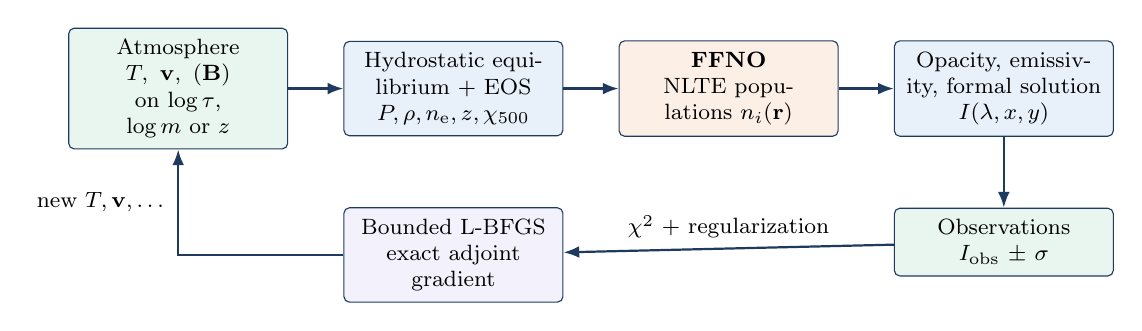
\begin{tikzpicture}[node distance=5mm and 7mm]
\node[box,fill=boxc,text width=25mm](a){Atmosphere\\$T,\ \mathbf v,\ (\mathbf B)$\\on $\log\tau$, $\log m$ or $z$};
\node[box,right=of a,text width=25mm](b){Hydrostatic equilibrium + EOS\\$P,\rho,\nel,z,\chi_{500}$};
\node[box,fill=boxb,right=of b,text width=25mm](c){\textbf{FFNO}\\NLTE populations $n_i(\mathbf r)$};
\node[box,right=of c,text width=25mm](d){Opacity, emissivity, formal solution\\$I(\lambda,x,y)$};
\node[box,fill=boxc,below=9mm of d,text width=25mm](e){Observations\\$I_{\rm obs}\pm\sigma$};
\node[box,fill=boxd,below=9mm of b,text width=25mm](f){Bounded L-BFGS\\exact adjoint gradient};
\draw[arr](a)--(b);\draw[arr](b)--(c);\draw[arr](c)--(d);\draw[arr](d)--(e);\draw[arr](e)--node[above,font=\footnotesize]{$\chi^2$ + regularization}(f);\draw[arr](f.west)-|node[left,font=\footnotesize,pos=.75]{new $T,\mathbf v,\dots$}(a.south);
\end{tikzpicture}
\caption{The chain. Orange is the learned step, blue is physics that is computed, green is data, and the lower loop runs only in inversion mode.}\label{fig:chain}
\end{figure}

\section{Radiative transfer}

\subsection{The transfer equation}
Along a ray with path length $s$, the specific intensity $I_\nu$ changes by what the gas emits minus what it absorbs:
\begin{equation}
\frac{\dd I_\nu}{\dd s}=\eta_\nu-\chi_\nu I_\nu ,
\end{equation}
with $\chi_\nu$ the extinction per unit length [m$^{-1}$] and $\eta_\nu$ the emissivity. Define the optical depth $\dd\tau_\nu=\chi_\nu\,\dd s$, measured toward the observer's side, and the source function $S_\nu=\eta_\nu/\chi_\nu$. The transfer equation then has the formal solution for the emergent intensity,
\begin{equation}
I_\nu(0)=I_\nu(\tau_{\rm b})\,e^{-\tau_{\rm b}}+\int_0^{\tau_{\rm b}}S_\nu(\tau)\,e^{-\tau}\,\dd\tau .\label{eq:formal}
\end{equation}
Two facts follow. The observed intensity is a weighted mean of the source function, with most of the weight around $\tau_\nu\approx1$; this is the sense in which a wavelength ``forms at a height''. And the height depends on wavelength: in the core of a strong line $\chi_\nu$ is large, so $\tau_\nu=1$ lies high, and in the wings it lies low. A line profile therefore samples the atmosphere in depth.

\subsection{Reference optical depth}
The continuum optical depth at 500\,nm, $\tau_{500}$, is the standard vertical coordinate. It is defined by the 500\,nm extinction $\chi_{500}$, integrated downward from the top, and $\tau_{500}=1$ marks the visible surface. Inversions naturally work on this axis, because that is where the data have sensitivity. It is a reference surface only: spectral lines form over their own ranges of $\tau_{500}$.

\subsection{Column mass}
A third vertical coordinate is column mass, $m=\int\rho\,\dd s$ [kg\,m$^{-2}$], the mass above a point per unit area. 1D semi-empirical models such as FAL-C are tabulated on it, because hydrostatic equilibrium is trivial on this axis: $P=g\,m$. The code supports all three axes (Section~\ref{sec:equilibrium}).

\section{Level populations: LTE and NLTE}

\subsection{LTE}
In local thermodynamic equilibrium the populations depend only on local $T$ and $\nel$. Within an ionization stage they follow Boltzmann's law, and between stages Saha's:
\begin{equation}
\frac{n_j^*}{n_i^*}=\frac{g_j}{g_i}\,e^{-(E_j-E_i)/kT},\qquad
\frac{n^*_{\rm c}\,\nel}{n^*_{i}}=\frac{2g_{\rm c}}{g_i}\left(\frac{2\pi m_{\rm e}kT}{h^2}\right)^{3/2}e^{-(E_{\rm c}-E_i)/kT}.
\end{equation}
For a line, LTE gives $S_\nu=B_\nu(T)$, the Planck function. All the difficulty below comes from this no longer being true.

\subsection{Statistical equilibrium}
In general the population of level $i$ is set by the balance of all transitions into and out of it. In a steady state,
\begin{equation}
\sum_{j\neq i}n_j\,(R_{ji}+C_{ji})=n_i\sum_{j\neq i}(R_{ij}+C_{ij}),\label{eq:se}
\end{equation}
with $C_{ij}$ the collisional rates, which depend locally on $T$ and $\nel$. The radiative rates depend on the radiation field. For a bound--bound transition between a lower level $l$ and an upper level $u$,
\begin{equation}
R_{ul}=A_{ul}+B_{ul}\bar J,\qquad R_{lu}=B_{lu}\bar J,\qquad
\bar J=\frac{1}{4\pi}\oint\!\!\int\phi(\nu,\mathbf n)\,I_\nu(\mathbf n)\,\dd\nu\,\dd\Omega ,
\end{equation}
where $\phi$ is the line profile, which includes the Doppler shift by the local velocity along direction $\mathbf n$.

Here is the coupling. $\bar J$ at a point depends on $I_\nu$ arriving from every direction, $I_\nu$ depends on $S_\nu$ and $\chi_\nu$ along those rays, and those depend on the populations there. In 3D, every point is coupled to every other point it can see within a few photon mean free paths. The result is non-local and nonlinear.

\subsection{Why this is non-local: a two-level illustration}
For a two-level atom with complete redistribution, Eq.~\eqref{eq:se} reduces to the classical line source function
\begin{equation}
S=(1-\varepsilon)\,\bar J+\varepsilon\,B_\nu(T),\qquad \varepsilon\approx\frac{C_{ul}}{C_{ul}+A_{ul}} .
\end{equation}
When collisions dominate, $\varepsilon\to1$ and $S\to B$: this is LTE. In the chromosphere $\varepsilon$ can be very small, so the source function is mostly $\bar J$, and it decouples from the local temperature. A photon scatters many times before being destroyed, and information travels over the thermalization length, which can greatly exceed the local scale height.

\subsection{Departure coefficients}
The conventional measure of the deviation from LTE is the departure coefficient,
\begin{equation}
b_i=\frac{n_i}{n_i^*}.
\end{equation}
Deep in the atmosphere $b_i\to1$. It is a useful diagnostic, and the training code can reconstruct it, but it is \emph{not} the network's output; see Section~\ref{sec:target}.

\subsection{The cost}
The established 3D solvers iterate Eq.~\eqref{eq:se}: formal solutions along many rays at many frequencies through the whole cube, then a population update, typically with accelerated lambda iteration. MULTI3D, which supplies the training labels here, does this with domain decomposition, and a large cube needs a supercomputer allocation. An inversion needs many forward evaluations, each of which would contain this calculation. That is the bottleneck FFNO removes.

\section{Model atoms and lines}

Each species has its own FFNO model, with six output channels. The levels and energies of the two atoms used in training and synthesis are in Table~\ref{tab:atoms}.

\begin{table}[H]\centering\small
\begin{tabular}{clr@{\hspace{2cm}}clr}
\toprule
\multicolumn{3}{c}{Hydrogen, \code{atom.h6_tiago2.yaml}}&\multicolumn{3}{c}{Calcium, \code{atom.ca2.yaml}}\\
Ch.&Level&$E$ [cm$^{-1}$]&Ch.&Level&$E$ [cm$^{-1}$]\\\midrule
1&H\,\textsc{i} $n=1$&0.000&1&Ca\,\textsc{ii} 4s $^2$S$_{1/2}$&0.000\\
2&H\,\textsc{i} $n=2$&82\,257.172&2&Ca\,\textsc{ii} 3d $^2$D$_{3/2}$&13\,650.248\\
3&H\,\textsc{i} $n=3$&97\,489.992&3&Ca\,\textsc{ii} 3d $^2$D$_{5/2}$&13\,710.900\\
4&H\,\textsc{i} $n=4$&102\,821.219&4&Ca\,\textsc{ii} 4p $^2$P$_{1/2}$&25\,191.535\\
5&H\,\textsc{i} $n=5$&105\,288.859&5&Ca\,\textsc{ii} 4p $^2$P$_{3/2}$&25\,414.465\\
6&H\,\textsc{ii} (protons)&109\,754.578&6&Ca\,\textsc{iii} ground term&95\,751.870\\\bottomrule
\end{tabular}
\caption{The six levels of each model atom. The last channel is the next ionization stage, so the network also predicts the ionization balance.}\label{tab:atoms}
\end{table}

\begin{figure}[H]\centering
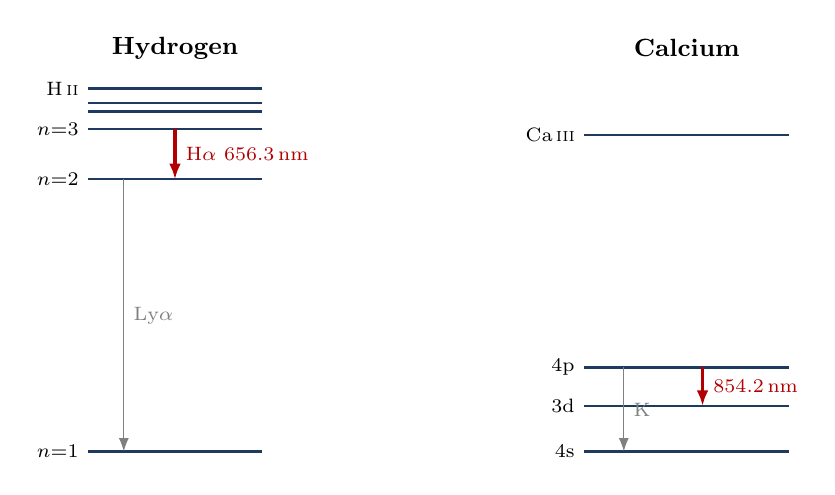
\begin{tikzpicture}[x=1cm,y=0.42mm]
\foreach \y/\l in {0/{$n{=}1$},82.26/{$n{=}2$},97.49/{$n{=}3$},102.82/{},105.29/{},109.75/{H\,\textsc{ii}}}{\draw[thick,ink](0,\y)--(2.2,\y);\node[font=\scriptsize,anchor=east]at(0,\y){\l};}
\draw[-{Latex[length=2mm]},red!70!black,very thick](1.1,97.49)--(1.1,82.26)node[midway,right,font=\scriptsize]{\Halpha{} 656.3\,nm};
\draw[-{Latex[length=1.7mm]},black!50](.45,82.26)--(.45,0)node[midway,right,font=\scriptsize]{Ly$\alpha$};
\node[font=\small\bfseries]at(1.1,122){Hydrogen};
\begin{scope}[xshift=6.3cm]
\foreach \y/\l in {0/{4s},13.65/{},13.71/{3d},25.19/{},25.41/{4p},95.75/{Ca\,\textsc{iii}}}{\draw[thick,ink](0,\y)--(2.6,\y);\node[font=\scriptsize,anchor=east]at(0,\y){\l};}
\draw[-{Latex[length=2mm]},red!70!black,very thick](1.5,25.41)--(1.5,13.71)node[midway,right,font=\scriptsize]{854.2\,nm};
\draw[-{Latex[length=1.7mm]},black!50](.5,25.41)--(.5,0)node[midway,right,font=\scriptsize]{K};
\node[font=\small\bfseries]at(1.3,122){Calcium};
\end{scope}
\end{tikzpicture}
\caption{Level diagrams to scale in energy (thousands of cm$^{-1}$). Red marks the line synthesized from FFNO populations: \Halpha{} uses channels 2 and 3 of the H model, and Ca\,\textsc{ii} 854.2\,nm uses channels 3 and 5 of the Ca model.}
\end{figure}

\Halpha{} opacity comes from the small population of $n=2$, which sits 10.2\,eV above the ground state and depends strongly on the Lyman radiation field and on the ionization state. Ca\,\textsc{ii} 854.2\,nm starts from a metastable level, and Ca is mostly ionized once to Ca\,\textsc{ii} in the chromosphere and further to Ca\,\textsc{iii} above. These populations are hard to predict in different ways, which is partly why the two species behave differently under validation (Section~\ref{sec:validation}).

\section{The training labels}\label{sec:labels}

\subsection{Atmospheres and solver}
The atmospheres are snapshots of 3D radiation-MHD simulations computed with Bifrost. MULTI3D then computes the NLTE populations in each snapshot. Those populations are the ground truth. The training pairs are:
\begin{equation*}
\underbrace{T(\mathbf r),\ \mathbf v(\mathbf r),\ \nel(\mathbf r),\ \rho(\mathbf r),\ z}_{\text{from the simulation}}
\quad\longrightarrow\quad
\underbrace{n_i(\mathbf r)}_{\text{from MULTI3D}} .
\end{equation*}
In the \code{_hion} simulations, the hydrogen ionization of the simulation is not in equilibrium and the atmosphere file carries the simulation's own hydrogen density.

\begin{table}[H]\centering\small
\begin{tabular}{llrrrrr}
\toprule
Simulation&Train / validation snapshot&$n_x{\times}n_y{\times}n_z$&$\Delta x$ [km]&$z$ range [Mm]&$\Delta z$ [km]\\\midrule
\code{en024048_hion}&465 / 700&$252^2\times467$&95.2&$-1.02$ to 14.37&18.6--97.1\\
\code{nw012023}&915 / 940&$256^2\times350$&46.9&$-0.97$ to 14.30&24.6--162.2\\
\code{ch012012_hion}&910 / 984&$256^2\times256$&46.9&$-2.45$ to 7.98&24.7--141.0\\
\code{ch012006}&836 / 849&$256^2\times256$&46.9&$-2.45$ to 7.98&24.7--141.0\\
\code{qs006003_sap}&689 / 900&$256^2\times256$&23.4&$-2.51$ to 0.62&12.3\\\bottomrule
\end{tabular}
\caption{Training and validation data: one snapshot per simulation for each. Grids were read from the mesh files. Further labelled snapshots, including the $384^3$ boxes \code{ch024031_by200bz005} and \code{en024031_by100_helium} ($-2.49$ to 14.30\,Mm, $\Delta x=62.5$\,km), are used only for evaluation.}\label{tab:sims}
\end{table}

The set deliberately covers different magnetic regimes and resolutions, and the vertical grids are all non-uniform in a similar way: fine through the lower atmosphere and stretched above. This matters later: the network has only ever seen such grids.

\subsection{Patches and scales}
Each snapshot is cut into patches of $40\times40$ columns with stride 20, at horizontal coarsening factors $s=1,\dots,8$ with an anti-alias Gaussian ($\sigma=s/2$ pixels). Only factors 1 to 6 actually yield a 40-pixel patch from a 256-pixel box, giving 161 patches per simulation. Coarsening gives the operator examples of the same physics at a different horizontal spacing $\Delta x\to s\Delta x$. The depth axis is always kept whole, at its native resolution.

\section{What the network learns}\label{sec:target}

\subsection{The operator}
The object learned is a map between functions on a volume, not a pointwise regression:
\begin{equation}
\mathcal G:\ \big(\log_{10}T,\ v_x,\ v_y,\ v_z,\ \log_{10}\nel,\ \log_{10}\rho\big)(\mathbf r)\ ,\ z,\ \Delta x,\ \Delta y\ \ \longmapsto\ \ \log_{10}n_i(\mathbf r),\quad i=1\dots6 .
\end{equation}
The output at one point depends on the input everywhere in the box, as it must physically.

\subsection{The inputs, and why each one is there}
\begin{table}[H]\centering\small
\begin{tabularx}{\linewidth}{lrrY}
\toprule
Channel&Mean&Std&Physical role\\\midrule
$\log_{10}T$ [K]&4.555&0.867&Sets collisional rates, Boltzmann and Saha factors, thermal Doppler width, and the local Planck source.\\
$v_x,v_y,v_z$ [km\,s$^{-1}$]&$-0.084,-0.040,0.540$&6.316, 5.316, 7.200&Velocity gradients shift line profiles between points, so they change how much radiation each point absorbs ($\bar J$).\\
$\log_{10}\nel$ [m$^{-3}$]&17.73&3.616&Collisional rates with electrons, and recombination.\\
$\log_{10}\rho$ [kg\,m$^{-3}$]&$-7.977$&4.059&Sets the element density and so the amount of absorbing matter.\\
\bottomrule
\end{tabularx}
\caption{Input channels with the normalization of the production checkpoints (identical for H and Ca). The large standard deviations reflect the many decades between the photosphere and the corona. All channels are standardized to zero mean and unit variance.}
\end{table}

Three geometric quantities also enter: the heights $z$ [Mm], and the horizontal spacings $\Delta x$, $\Delta y$ [m], since the optical thickness between two points depends on their physical separation.

Two quantities are deliberately absent. The \textbf{magnetic field} is not an input, because the populations here are computed without magnetic effects on the atomic rates; $\mathbf B$ acts only indirectly, through the $T$, $\rho$ and $\mathbf v$ it has shaped. \textbf{Microturbulence} $\vturb$ is not an input, so populations do not respond to it, even though it broadens lines in synthesis.

\subsection{The target: log populations, not departure coefficients}
The network's output channels are standardized values of $\log_{10}n_i$, with $n_i$ in m$^{-3}$. The code's earlier target was $\log_{10}b_i$, and some old notes and variable names (\code{logb}) still say so, but the production checkpoints and datasets store \code{log10_nlte_population_m-3}. Logarithms are essential because a single level spans many decades:

\begin{table}[H]\centering\small
\begin{tabular}{l*{6}{r}}
\toprule
Mean $\pm$ std of $\log_{10}n_i$ [m$^{-3}$]&ch.\,1&ch.\,2&ch.\,3&ch.\,4&ch.\,5&ch.\,6\\\midrule
Hydrogen&$16.02\pm6.87$&$9.64\pm8.02$&$8.66\pm8.11$&$8.51\pm8.10$&$8.49\pm8.13$&$17.63\pm3.67$\\
Calcium&$11.32\pm5.34$&$10.39\pm5.52$&$10.58\pm5.50$&$8.60\pm6.06$&$8.87\pm6.06$&$12.30\pm3.73$\\
\bottomrule
\end{tabular}
\caption{Target normalization from the production checkpoints.}
\end{table}

One consequence needs stating directly. A prediction in $\log_{10}n_i$ has no built-in constraint on the element total: the sum $\sum_i n_i$ should equal the element density, which follows from $\rho$ and the abundance, but the network only learns this approximately. The difference needs no labels to compute and turns out to be a useful error indicator (Section~\ref{sec:validation}).

\section{The architecture, read physically}

The model is a factorized Fourier neural operator. A general 3D convolution or 3D Fourier layer treats all three axes alike, but the problem does not: the atmosphere is strongly stratified and has a non-uniform $z$ grid, while horizontally it is statistically homogeneous and periodic. So each block splits its update into a horizontal part and a vertical part.

\begin{figure}[H]\centering
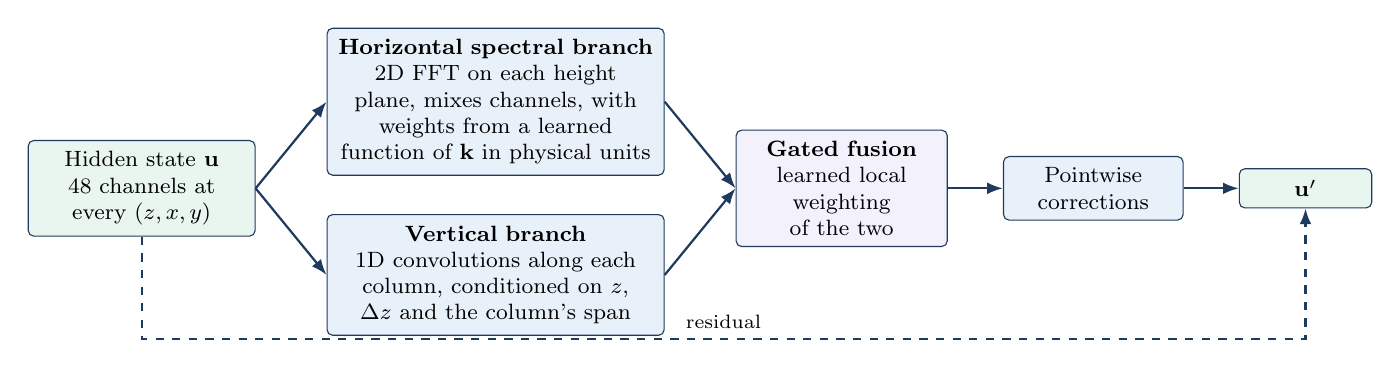
\begin{tikzpicture}[node distance=4mm and 5mm]
\node[box,fill=boxc,text width=26mm](x){Hidden state $\mathbf u$\\48 channels at every $(z,x,y)$};
\node[box,right=9mm of x,yshift=11mm,text width=40mm](s){\textbf{Horizontal spectral branch}\\2D FFT on each height plane, mixes channels, with weights from a learned function of $\mathbf k$ in physical units};
\node[box,right=9mm of x,yshift=-11mm,text width=40mm](v){\textbf{Vertical branch}\\1D convolutions along each column, conditioned on $z$, $\Delta z$ and the column's span};
\node[box,fill=boxd,right=9mm of s,yshift=-11mm,text width=24mm](f){\textbf{Gated fusion}\\learned local weighting of the two};
\node[box,right=7mm of f,text width=20mm](p){Pointwise corrections};
\node[box,fill=boxc,right=7mm of p,text width=14mm](o){$\mathbf u'$};
\draw[arr](x.east)--(s.west);\draw[arr](x.east)--(v.west);\draw[arr](s.east)--(f.west);\draw[arr](v.east)--(f.west);\draw[arr](f)--(p);\draw[arr](p)--(o);
\draw[arr,dashed](x.south)--++(0,-13mm)-|node[pos=.25,above,font=\scriptsize]{residual}(o.south);
\end{tikzpicture}
\caption{One block. Four such blocks sit between a pointwise lift from 6 to 48 channels and a pointwise projection to the 6 output channels. Total: 3.12 million parameters.}\label{fig:block}
\end{figure}

\subsection{Horizontal branch: radiation coupling across columns}
On each height plane, independently of the others, the state is Fourier transformed in $(x,y)$ and multiplied in spectral space:
\begin{equation}
\hat u'_o(\mathbf k,z)=g(\mathbf k)\sum_i W_{io}\,\hat u_i(\mathbf k,z),\qquad g(\mathbf k)=\mathrm{MLP}\big(k_x,k_y,|\mathbf k|,\mathrm{sign}\,k_y\big)\in\mathbb C,
\end{equation}
where $W$ is a complex channel-mixing matrix. A multiplication at each $\mathbf k$ is a convolution over the whole plane in real space, so one layer communicates across the entire box. This is the structure of the real problem: a horizontally uniform layer's response to a perturbation depends on its horizontal scale, because small-scale structure is smoothed by radiative exchange and large-scale structure is not. Since $g$ is a function of the wavenumber in physical units (m$^{-1}$), not of a mode number, the same weights apply to any grid size and spacing. This is what makes a model trained on $40\times40$ patches applicable to whole cubes.

\subsection{Vertical branch: stratification and optical depth}
Along each column, a stack of 1D convolutions processes the state (three parallel kernels 3, 7 and 15 points wide, then residual blocks with dilations 1, 2 and 4, then a block of kernel 7), and it is given the column's geometry: absolute height $z$, normalized height $(z-z_{\rm min})/z_{\rm span}$, local spacing $\Delta z/\langle\Delta z\rangle$ and the span $z_{\rm span}$. These are the terms that replace an explicit optical-depth integration. The filters run over grid \emph{index}, so physical distance enters only through these features.

This design has a consequence the physics depends on: the network sees index-based stencils and whole-column descriptors, so it is sensitive to how the column is sampled and how far it extends, and it should only be used on grids resembling its training grids. Section~\ref{sec:mesh} builds exactly such a grid.

\subsection{Fusion and local corrections}
A sigmoid gate, computed pointwise from the state and both branch outputs, decides how much of each branch to use at each location. This lets the network favour vertical information in optically thick, stratified layers and horizontal information elsewhere, though the weights are learned rather than imposed. A small $3\times3\times3$ depthwise convolution inside the fusion adds a short-range coupling. Two further pointwise terms provide local nonlinearity, which is what thermodynamic relations such as Saha and Boltzmann are. The learned residual weights in the production H checkpoint are about 0.76--0.92 for the fused update and 0.15--0.20 for each pointwise term, so the combined spectral and vertical update dominates.

\subsection{What the network does not have}
It contains no radiative transfer equation, no statistical equilibrium and no explicit atomic data. Physics enters through the data, the choice of inputs and outputs, and the factorization.

\section{The training objective}
Over normalized targets $y$, with prediction $\hat y$, the data term is
\begin{equation}
\mathcal L=\tfrac12\,\big\langle(1+|y|)(\hat y-y)^2\big\rangle+\tfrac12\,\big\langle|\hat y-y|\big\rangle .
\end{equation}
The $L^1$ part reduces sensitivity to outliers, and the factor $1+|y|$ puts more weight on values far from the mean, meaning extreme populations. The code can also compute a term on the line source-function exponent,
\begin{equation}
x_{lu}=\ln\frac{b_l}{b_u}+\frac{E_u-E_l}{kT},\qquad S_\nu=\frac{2h\nu^3}{c^2}\,\frac{1}{e^{x_{lu}}-1},
\end{equation}
and a horizontal-gradient term. \emph{Both have weight zero in production:} the source term is computed and logged as a monitor, but the checkpoints were optimized on the data term alone. Conservation is not enforced either. The production checkpoints reached validation losses of $5.9\times10^{-3}$ (H, best epoch 171) and $7.3\times10^{-3}$ (Ca, best epoch 252), with training losses $4.3\times10^{-3}$ and $3.6\times10^{-3}$.

\section{From a temperature to a full atmosphere}\label{sec:equilibrium}

An inversion's unknowns are $T$, $\mathbf v$, $\vturb$ and $\mathbf B$. FFNO also needs $\nel$, $\rho$ and $z$. These come from assuming each column is in \textbf{hydrostatic equilibrium}, with a separate code, HSEMHS, as the only authority:
\begin{equation}
\frac{\dd P}{\dd z}=-\rho g,\qquad \rho=\rho(T,P),\quad \nel=\nel(T,P),\quad\chi_{500}=\chi_{500}(T,P),\qquad g=274\ \mathrm{m\,s^{-2}}.
\end{equation}
The equation of state is Wittmann's LTE EOS with solar abundances, tabulated in $(\ln T,\ln P)$.

\subsection{Three vertical axes}
\begin{table}[H]\centering\small
\begin{tabularx}{\linewidth}{lYYY}
\toprule
&Native $\log_{10}\tau_{500}$&Native $\log_{10}m$&Native $z$\\\midrule
Equations&$\dfrac{\dd\ln P}{\dd\ln\tau}=\dfrac{g\tau\rho}{\chi P}$,\quad $\dfrac{\dd z}{\dd\ln\tau}=-\dfrac{\tau}{\chi}$&$P=g\,m$,\quad $\dd z=-\dd m/\rho$&$\dfrac{\dd\ln P}{\dd z}=-\dfrac{\rho g}{P}$\\[3mm]
Boundary&Top closure $P_{\rm top}=g\,\tau_{\rm top}/\kappa_{\rm top}$, with $\kappa=\chi/\rho$ constant above the top level&None needed&One prescribed pressure at an anchor level\\
Derived&$P,\rho,\nel,\chi_{500},z$&$P,\rho,\nel,\chi_{500},z,\tau_{500}$&$P,\rho,\nel,\chi_{500},\tau_{500}$\\
Column offsets&Equal $P+B^2/2\mu_0$ at one height, mean $z(\tau=1)=0$&The same kind of alignment&Heights given\\
\bottomrule
\end{tabularx}
\caption{The equilibrium on each native axis (no magnetic field in the force balance). At $\mu<1$ the $\tau$ and $m$ axes count along the ray, so that $P=\mu g m$.}
\end{table}

The total-pressure alignment is a lateral force balance that ignores magnetic tension, so absolute heights are gauge-dependent. Column hydrostatic equilibrium is a model of a dynamic atmosphere: it does not hold in shocks and is a real source of error (Section~\ref{sec:validation}). Magnetohydrostatic modes exist in HSEMHS but are not yet connected to the FFNO path.

\subsection{Giving the electron density}
The LTE EOS can be far from a model's real $\nel$. For FAL-C the tabulated $\nel$ differs from the EOS value by about 9\% in the photosphere and a factor of about 2.6 near 1\,Mm, which alone moves the RH Ca\,\textsc{ii} 854.2\,nm core from 0.81 to $1.45\times10^{-8}$ SI and adds a self-reversal. So \emph{in forward synthesis only}, $\nel$ can be supplied as the truth. $P$ then becomes the pressure at which the EOS gives this $\nel$ at this $T$, and $\rho$ and $\chi_{500}$ follow. No hydrostatic integration is done, and $P$ and $\rho$ can be far from the model's, because the EOS is LTE. Inversions always take $\nel$ from the EOS.

\subsection{Giving the whole atmosphere}
With $\nel$ and hydrogen populations both supplied, HSEMHS is not used. As in RH,
\begin{gather}
n_{\rm H}=\sum_i n_i,\qquad \rho=m_{\rm per\,H}\,n_{\rm H},\qquad P=\big(n_{\rm H}\sum_j A_j+\nel\big)kT,
\end{gather}
with Wittmann's composition ($m_{\rm per\,H}=2.3397\times10^{-27}$\,kg, $\sum_j A_j=1.0950$). $\chi_{500}$ comes from the continuum model at 500\,nm with the given hydrogen. Heights follow per column, with every column gauged to $z(\tau=1)=0$:
\begin{align}
\log m\text{ axis:}&\quad \dd z_k=-\frac{2\mu\,\Delta m}{\rho_{k-1}+\rho_k},\quad \tau_1=\frac{\chi_{500}}{\rho}m_1,\quad\dd\tau=\frac{\chi_{500,k-1}+\chi_{500,k}}{2}\frac{|\dd z|}{\mu},\\
\log\tau\text{ axis:}&\quad \dd z_k=-\frac{2\mu\,\Delta\tau}{\chi_{500,k-1}+\chi_{500,k}},\\
z\text{ axis:}&\quad\text{the axis itself, with }\tau_1=\chi_{500,1}|\Delta z|/(2\mu)\text{, or 0 if that exceeds 1.}
\end{align}
FFNO still predicts the line populations in this mode. This route exists for comparisons with 1D codes on the same model.

\section{The population mesh}\label{sec:mesh}

\subsection{Why it is needed}
FFNO has seen only height grids that are one set of heights for every column, spaced 12--30\,km through the photosphere and chromosphere, with bottoms 1--2.5\,Mm below the surface and tops up to 14\,Mm. A typical inversion column has 95 log-$\tau$ points spaced from 30\,km to several Mm, at different heights in each column. Fed directly, H $n=2$ comes out about 100 times wrong in the chromosphere, even with the simulation's own $T$, $\mathbf v$, $\nel$ and $\rho$. The fix is to \emph{bring the atmosphere to the network} rather than asking it to extrapolate.

\subsection{Construction}
The default mesh has 452 levels running from $-1$\,Mm to 14\,Mm: 20\,km spacing to 4.5\,Mm, then growing by 1\% per point up to 100\,km. Then, for each column:

\begin{figure}[H]\centering
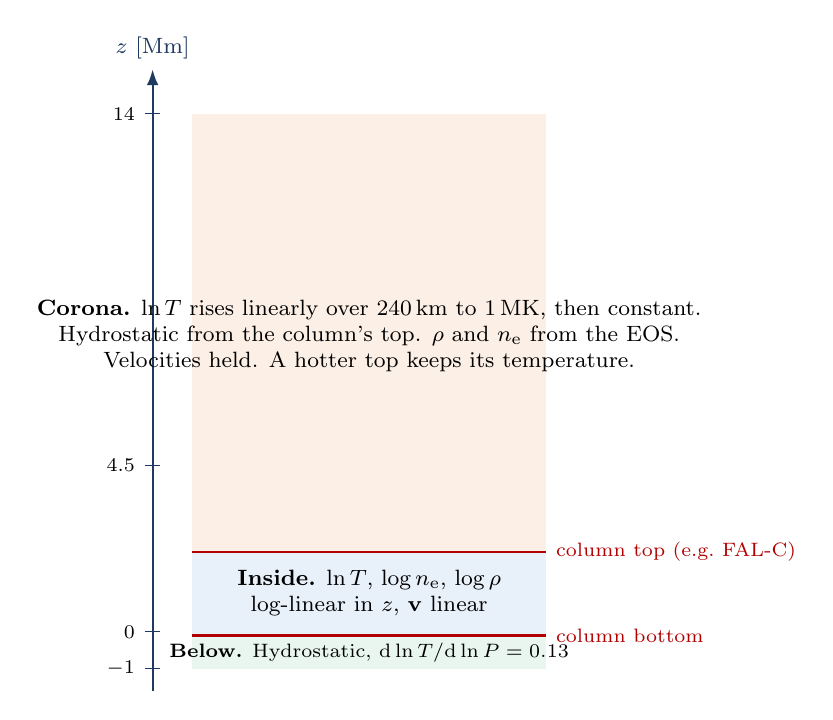
\begin{tikzpicture}[x=1cm,y=4.7mm]
\draw[-{Latex[length=2mm]},ink,thick](0,-1.6)--(0,15.2)node[above,font=\footnotesize]{$z$ [Mm]};
\foreach \z in {0,4.5,14}{\draw[ink](-.1,\z)--(.1,\z);\node[font=\scriptsize,anchor=east]at(-.1,\z){\z};}
\draw[ink](-.1,-1)--(.1,-1);\node[font=\scriptsize,anchor=east]at(-.1,-1){$-1$};
\fill[boxb](.5,2.16)rectangle(5,14);\fill[boxa](.5,-.1)rectangle(5,2.16);\fill[boxc](.5,-1)rectangle(5,-.1);
\node[font=\footnotesize,align=center]at(2.75,8){\textbf{Corona.} $\ln T$ rises linearly over 240\,km to 1\,MK, then constant.\\Hydrostatic from the column's top. $\rho$ and $\nel$ from the EOS.\\Velocities held. A hotter top keeps its temperature.};
\node[font=\footnotesize,align=center]at(2.75,1.05){\textbf{Inside.} $\ln T$, $\log\nel$, $\log\rho$\\log-linear in $z$, $\mathbf v$ linear};
\node[font=\scriptsize]at(2.75,-.55){\textbf{Below.} Hydrostatic, $\dd\ln T/\dd\ln P=0.13$};
\draw[thick,red!70!black](.5,2.16)--(5,2.16);\node[font=\scriptsize,anchor=west,red!70!black]at(5,2.16){column top (e.g.\ FAL-C)};
\draw[thick,red!70!black](.5,-.1)--(5,-.1);\node[font=\scriptsize,anchor=west,red!70!black]at(5,-.1){column bottom};
\end{tikzpicture}
\caption{How one column fills the fixed mesh. Heights are illustrative of a 1D model reaching 2.16\,Mm.}
\end{figure}

The network predicts on the mesh, and the populations are interpolated back to the column's own points, log-linearly in $z$. The extensions exist \emph{only} for the network: synthesis uses the column's own levels. The mesh is on by default for log $\tau$ and log $m$, and optional on $z$, where it is needed for anything unlike a simulation grid.

\subsection{Why the corona matters}
Filling the volume above a short column is not a detail. The network is not local in height: populations low down respond to what occupies the mesh above. For FAL-C, holding its 100\,000\,K top values up to 14\,Mm made total hydrogen up to 15 times too high in the photosphere, and changing a corona from 1\,MK to 0.5\,MK doubled it at 250\,km. This reflects the operator's learned dependence on column context, not a physical influence of that gas on the photosphere; it is the same effect that appears as the column-span dependence in Section~\ref{sec:validation}. Columns already reaching the mesh top, like Bifrost cubes on log $\tau$, never use this extension.

\section{Spectral synthesis}

\subsection{FFNO lines}
With populations $n_l,n_u$ of the line's two levels, the line opacity and emissivity per wavelength interval are
\begin{equation}
\alpha_\lambda=\frac{hc}{4\pi\lambda_0}\,\phi_\lambda\,(n_lB_{lu}-n_uB_{ul}),\qquad j_\lambda=\frac{hc}{4\pi\lambda_0}\,\phi_\lambda\,n_uA_{ul},
\end{equation}
with the same profile in absorption and emission: \textbf{complete redistribution}, non-PRD. The profile is a Voigt function of
\begin{gather}
\phi_\lambda=\frac{H(a,|v|)}{\sqrt\pi\,\Delta\lambda_{\rm D}},\qquad v=\frac{\lambda-\lambda_{\rm c}+\lambda_0\vlos/c}{\Delta\lambda_{\rm D}},\qquad a=\frac{\gamma\lambda^2}{4\pi c\,\Delta\lambda_{\rm D}},\\
\Delta\lambda_{\rm D}=\frac{\lambda_0}{c}\sqrt{\frac{2kT}{m_{\rm atom}}+\vturb^2},\qquad \gamma=\gamma_{\rm nat}+\sum_p C_p\,T^{a_p}\,\nel^{b_p}\,n_{\rm H\,I}^{c_p}.
\end{gather}
Positive $\vlos$ (toward the observer) gives a blue shift. The sum over $p$ holds the atom file's Stark and van der Waals terms. Neutral hydrogen in the broadening comes from the EOS at $(T,P)$, not from FFNO: the only FFNO populations read by synthesis are the line's two levels.

\subsection{Line centres and wavelengths}
By default the profile centre $\lambda_{\rm c}$ is a reference: \Halpha{} at 656.28\,nm and Ca\,\textsc{ii} at 854.209\,nm in air, because the atom files' level energies put them about $+0.16$\,\AA{} and $-0.03$\,\AA{} away. Only the detuning moves; width and strength stay the atom's. The option \code{line_center = "atom"} uses the level energies instead.

Synthesis always runs on vacuum wavelengths, with air-to-vacuum conversion by Edl\'en's formula, as in RH's \code{air_to_vacuum}. Air is an input and output label only.

\subsection{The continuum}
Every spectral region has exactly one continuum, evaluated at its central wavelength:
\begin{equation}
\alpha_{\rm c}=\sigma_{\rm atoms}(T,\nel)\,n_{\rm H}+\sigma_{\rm H^-}(T)\,\nel\,n_{\rm H\,I}+\sigma_{\rm H\,ff}(T)\,\nel\,n_{\rm p}+\sigma_{\rm H_2^+}(T)\,n_{\rm p}\,n_{\rm H\,I}+\sigma_{\rm R}\,n_{\rm H\,I}+\sigma_{\rm T}\,\nel ,
\end{equation}
where the terms are bound--free absorption of 14 background atoms, H$^-$ bound--free and free--free, hydrogen free--free, H$_2^+$, Rayleigh scattering on H and Thomson scattering. The neutral hydrogen and protons come from the \textbf{EOS at $(T,P)$}, or from the input in a given atmosphere. \textbf{FFNO populations never enter the continuum}, forward or inverse. This keeps wing and continuum formation independent of population errors.

The emissivity is $j_{\rm c}=\alpha_{\rm c}B_\lambda(T)$, so scattering contributions are treated as if thermal; this is a simplification that makes the continuum local. Against RH on FAL-C, the continuum is about 1--4\% lower in the blue (422\,nm: $-3.7$\%, 788\,nm: $-1.0$\%), partly because this model includes H$_2^+$ bound--free opacity, which RH does not.

\subsection{LTE blends}
Other lines come from Kurucz lists in LTE: the lower level's population from the Wittmann EOS at $(T,P)$, the upper from Boltzmann, source function $B_\lambda(T)$. Their van der Waals broadening is, in order of preference, ABO given explicitly, ABO from tables for s--p, p--d and d--f transitions of neutral atoms, the list's value, or Uns\"old. Opacities and emissivities of all sources in a region are added before one formal solution, so blends such as Fe\,\textsc{i} 656.92\,nm near \Halpha{} and Si\,\textsc{i} 853.62\,nm near Ca\,\textsc{ii} are treated together. A Kurucz line that \emph{is} the FFNO transition is dropped.

\subsection{The formal solution}
The solver evaluates Eq.~\eqref{eq:formal} by short characteristics: starting at the bottom with $I=S$, it takes one step at a time with the source function linear in $\tau$ across the step of optical thickness $\Delta$,
\begin{equation}
I_k=e^{-\Delta}I_{k+1}+\Big(\frac{1-e^{-\Delta}}{\Delta}-e^{-\Delta}\Big)S_{k+1}+\Big(1-\frac{1-e^{-\Delta}}{\Delta}\Big)S_k .
\end{equation}
The choice of integration variable matters and depends on the axis:
\begin{align}
\log\tau\text{ axis:}&\quad \dd\tau_\lambda=\frac{\chi_\lambda}{\chi_{500}}\,\tau_{500}\,\dd\ln\tau_{500},\\
\log m\text{ axis:}&\quad \dd\tau_\lambda=\frac{\chi_\lambda}{\rho}\,m\,\dd\ln m,\\
z\text{ axis:}&\quad \dd\tau_\lambda=\chi_\lambda\,\dd z/\mu .
\end{align}
This is not cosmetic. A 0.1\,dex log-$\tau$ step can span the whole transition region, 9\,600\,km in one column of a production run. There, a trapezoid in height assigns the cool point's opacity to all of the hot gas, makes the step optically thick, and lets the emergent intensity be set by the corona. Integrating on the native axis avoids this. Additionally, any step where $\ln\chi$ or $\ln\eta$ changes by more than 1 is split into up to 256 substeps, log-linear inside, so a step across a huge jump does not give the hot end's source function a false weight.

\section{Viewing angle}
Away from disk centre, the ray has direction $\mathbf n=(\sin\theta\cos\phi,\sin\theta\sin\phi,\mu)$, with $\mu=\cos\theta$. Three things change: the Doppler shift uses $\vlos=\mathbf n\cdot\mathbf v$; the path is $\dd z/\mu$; and in the \code{inclined} geometry each ray passes through different columns, $\mathbf x=\boldsymbol\xi+\mathbf t\,z$, with $\mathbf t=\tan\theta\,(\cos\phi,\sin\phi)$.

The populations themselves come from a 3D solution, so they do not depend on the viewing angle. That is the advantage of predicting populations. What must be right is the \emph{geometry they are evaluated in}:
\begin{itemize}
\item \textbf{Native $z$:} the network sees the cube as it is; afterwards, state and populations are shifted by $+\mathbf t z$ per level onto the rays, and synthesis follows the rays.
\item \textbf{Native log $\tau$ or log $m$:} the input columns must already be rays. In \code{inclined} geometry, the mesh shifts each level by $-\mathbf t z$ to put every ray point at its true Cartesian position before the network, and the populations back by $+\mathbf t z$ afterwards.
\end{itemize}
Without that shift the network sees a tilted atmosphere as if vertical. The measured correlation of the network input with the true cube at 1200\,km, with and without the shift, is 0.55 and 0.02 in $T$; at 300\,km it is 0.96 and 0.68.

\begin{figure}[H]\centering
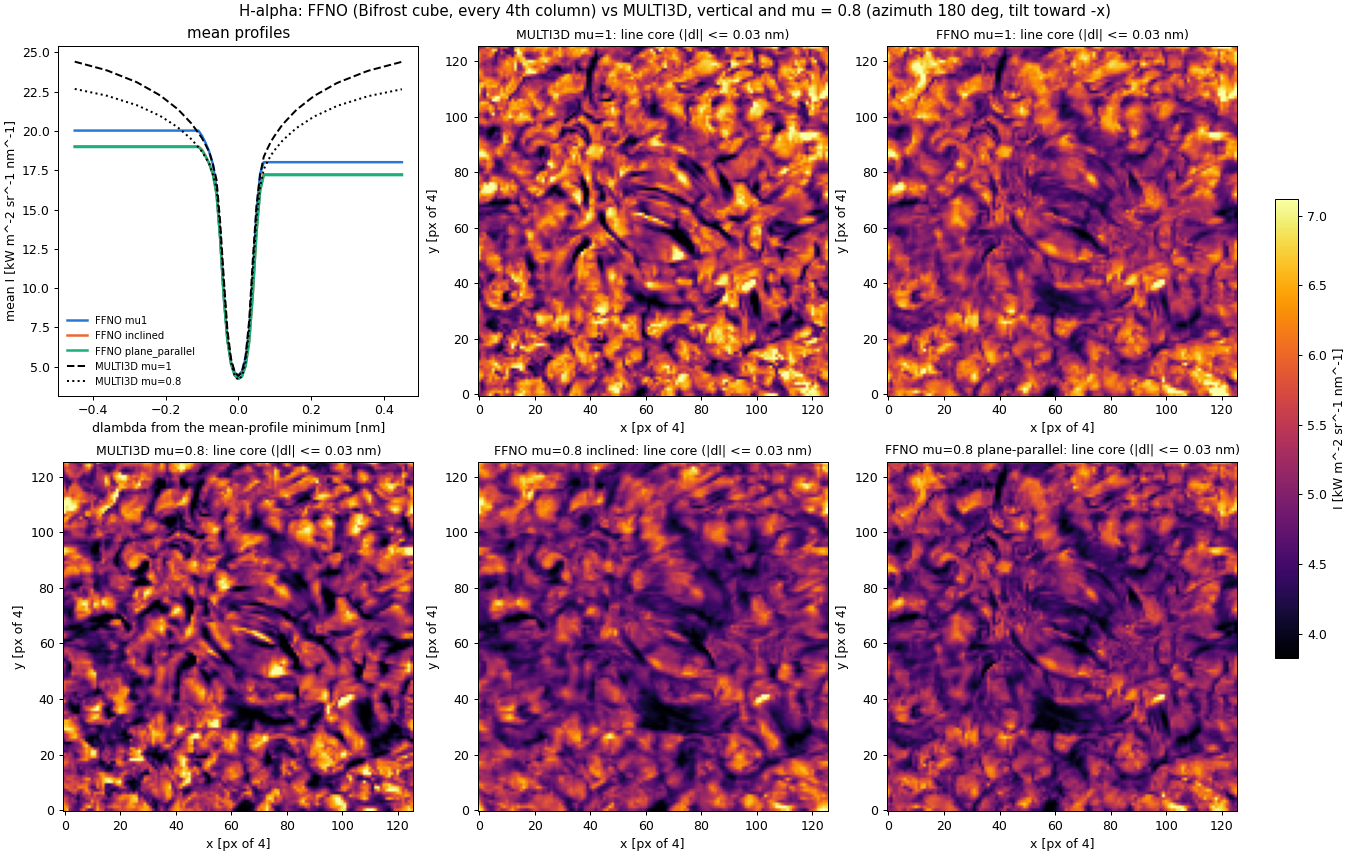
\includegraphics[width=.92\linewidth]{figures/ffno_vs_multi3d_mu08.png}
\caption{FFNO against MULTI3D at $\mu=1$ and $\mu=0.8$ on a Bifrost cube, \Halpha{} line-core maps. Inclined geometry gives $r=0.81$ against MULTI3D at $\mu=0.8$, comparable to $r=0.82$ at $\mu=1$. Plane-parallel synthesis gives $r=0.04$, so the geometry is essential.}
\end{figure}

\section{Inversion}

\subsection{The problem}
Given an observed cube $I_{\rm obs}(\lambda,x,y)$ with uncertainty $\sigma$, find the atmosphere that reproduces it, minimizing
\begin{equation}
J(\mathbf p)=\frac{1}{N}\sum_{\lambda,x,y}\Big(w\,\frac{I_{\rm syn}(\mathbf p)-I_{\rm obs}}{\sigma}\Big)^2+R(\text{atmosphere}).
\end{equation}
$I_{\rm syn}$ includes Gaussian spectral and spatial PSFs. All columns are one problem, coupled by the Fourier layers, the PSF and horizontal regularization; this is not a set of independent 1D fits.

\subsection{Unknowns}
The parameters $\mathbf p$ are physical values on coarse maps with a few vertical nodes, for $T$, velocity (or $\vlos$), $\vturb$ and $\mathbf B$. The atmosphere at each trial is
\begin{equation}
A=A_{\rm start}+\mathcal I\big(\mathbf p-\mathbf p_{\rm initial}\big),
\end{equation}
with $\mathcal I$ a trilinear expansion to the full grid. So the nodes carry only \emph{corrections}: fine structure in the starting atmosphere is preserved, and the first evaluation is that atmosphere itself. Bounds apply to the full field. An out-of-bounds trial is rejected, not clipped.

\subsection{Sensitivity: what the data constrain}
Which parts of the atmosphere the spectrum constrains is expressed by the response function $R_v(\lambda,k)=\partial I(\lambda)/\partial v(k)$. Figure~\ref{fig:rf} shows it for \Halpha: the core responds near $\log\tau_{500}\approx-6$, at the top of the chromosphere, and sometimes in a second, deeper layer; the wing responds near $\log\tau_{500}\approx-0.5$. FFNO and MULTI3D populations give the same picture.

\begin{figure}[H]\centering
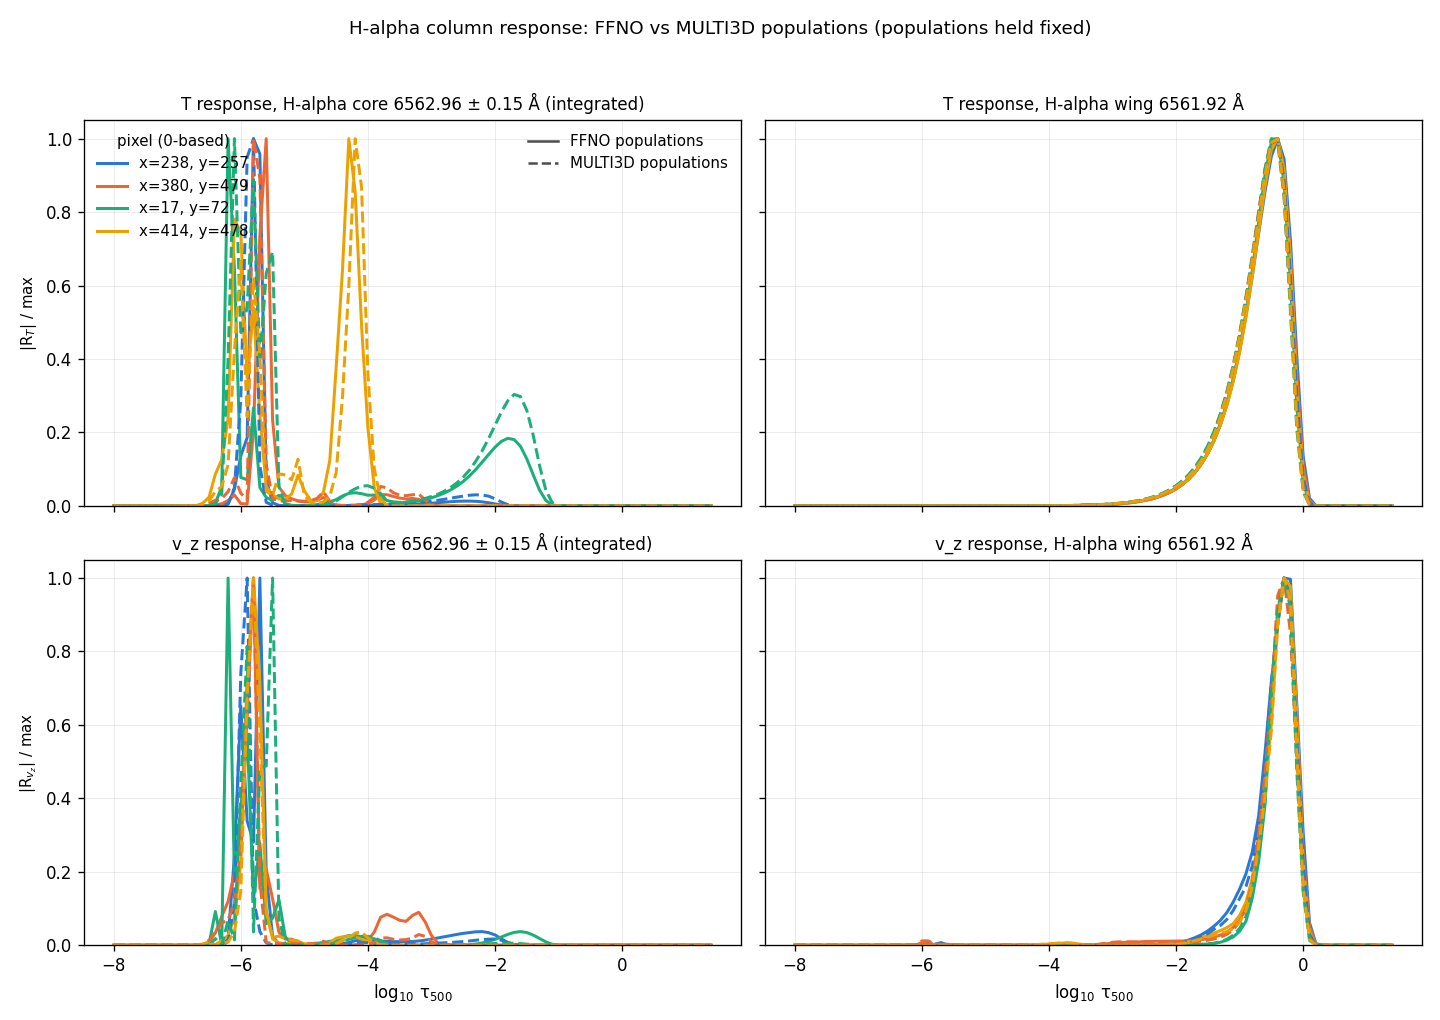
\includegraphics[width=.84\linewidth]{figures/ffno_vs_multi3d_halpha.png}
\caption{Response of \Halpha{} to temperature and $v_z$ in four columns, with populations held fixed at the FFNO (solid) or MULTI3D (dashed) values.}\label{fig:rf}
\end{figure}

There is a physical subtlety. With populations held fixed, the response in the line core is that of the opacity and the emissivity only. If populations are allowed to respond to $T$ through FFNO, one obtains the full derivative, including NLTE effects:
\begin{equation}
\frac{\dd I}{\dd T}=\frac{\partial I}{\partial T}\Big|_{n}+\sum_{l}\frac{\partial I}{\partial n_l}\frac{\partial n_l}{\partial T}.
\end{equation}
The second term contains the network's own derivative, which is not constrained directly by training: the training loss sees values, not Jacobians. How faithful $\partial n/\partial T$ is to the true NLTE response should be treated as an open question for each application.

\subsection{Gradient}
The objective's gradient comes from one reverse pass through the chain:
\begin{center}
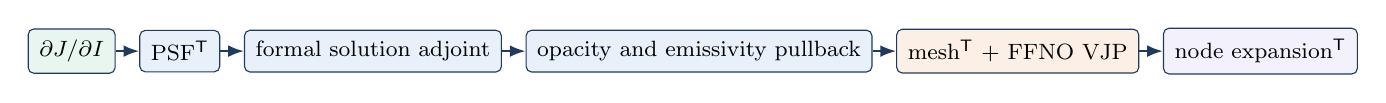
\begin{tikzpicture}[node distance=3mm]
\node[box,fill=boxc](a){$\partial J/\partial I$};\node[box,right=of a](b){PSF$^{\mathsf T}$};\node[box,right=of b](c){formal solution adjoint};\node[box,right=of c](d){opacity and emissivity pullback};\node[box,fill=boxb,right=of d](e){mesh$^{\mathsf T}$ + FFNO VJP};\node[box,fill=boxd,right=of e](f){node expansion$^{\mathsf T}$};
\draw[arr](a)--(b);\draw[arr](b)--(c);\draw[arr](c)--(d);\draw[arr](d)--(e);\draw[arr](e)--(f);
\end{tikzpicture}
\end{center}
The contribution of the hydrostatic equilibrium ($\partial P/\partial T$ and so on) and the regularization is added by centred finite differences per control coordinate. The transposes are exact and have been checked: gradient against finite differences to about $4\times10^{-10}$ on log $\tau$ and $3\times10^{-9}$ on $z$ at $\mu=0.8$. The result drives a bounded L-BFGS optimizer with Armijo backtracking.

\subsection{Regularization}
A real inversion is ill-posed: many atmospheres fit the same spectra, and layers outside the response function are unconstrained. The penalty has seven STiC-style vertical slots ($T$, $\vlos$, $\vturb$, $B$, inclination, azimuth, boundary pressure), each of which can penalize the first derivative, deviation from the depth mean, deviation from zero, or the second derivative, plus horizontal first or second differences per variable. It acts on the \emph{full} recovered atmosphere.

\section{How well it works: measurements}\label{sec:validation}

All numbers below come from runs in this repository. Note that every labelled snapshot has now been inspected during development, so there is no pristine test set. A final evaluation needs a new MULTI3D snapshot.

\subsection{Spectra against MULTI3D}
\begin{table}[H]\centering\small
\begin{tabular}{lrr}
\toprule
Case (true thermodynamics, on the simulation grid)&\Halpha{} core MAE&Ca\,\textsc{ii} 854.2 core MAE\\\midrule
\code{nw012023} 915 (training)&6.8\%&6.6\%\\
\code{nw012023} 940 (validation)&8.5\%&10.2\%\\
\code{nw012023} 1050&9.4\%&16.6\%\\
\code{nw012023} 1120&11.3\%&13.7\%\\
\code{en024048_hion} 700 (validation)&18.5\%, bias $+17$\%&20.7\%, bias $+18$\%\\
\code{ch012012_hion} 759&7.2\%&10.2\%\\\bottomrule
\end{tabular}
\caption{Line-core intensity error of synthesis from FFNO populations against synthesis from MULTI3D populations.}
\end{table}

Population errors and spectral errors are not monotonically related. In \code{ch012012_hion} 759, Ca\,\textsc{ii} is 1.3\,dex too low at 2--3\,Mm, the model over-ionizing it to Ca\,\textsc{iii}, yet the 854.2\,nm core changes by only 10\%. Conversely, in \code{en024048_hion} 700 moderate population errors make both cores 17--18\% too bright. So a good spectrum does not by itself certify the populations.

\subsection{The full route, with hydrostatic thermodynamics}
On \code{en024048_hion} 385 against MULTI3D (every fourth column): the log-$\tau$ hydrostatic route gives far wings within 1\%, an \Halpha{} core map correlation of $r=0.65$ and a Ca\,\textsc{ii} core correlation of $r=0.92$. On the cube's own height grid with the simulation's thermodynamics, the \Halpha{} core reaches $r=0.82$. The gap of 0.82 to 0.65 measures what the hydrostatic assumption and the log-$\tau$ route cost, not FFNO alone. With $\nel$ given on $z$, far wings are good ($r=0.99$ against 0.29 for hydrostatic $z$), but $P$ can be $10\times$ off at 1\,Mm and the \Halpha{} core falls to $r=0.23$.

\subsection{Against RH on a 1D model}
\begin{figure}[H]\centering
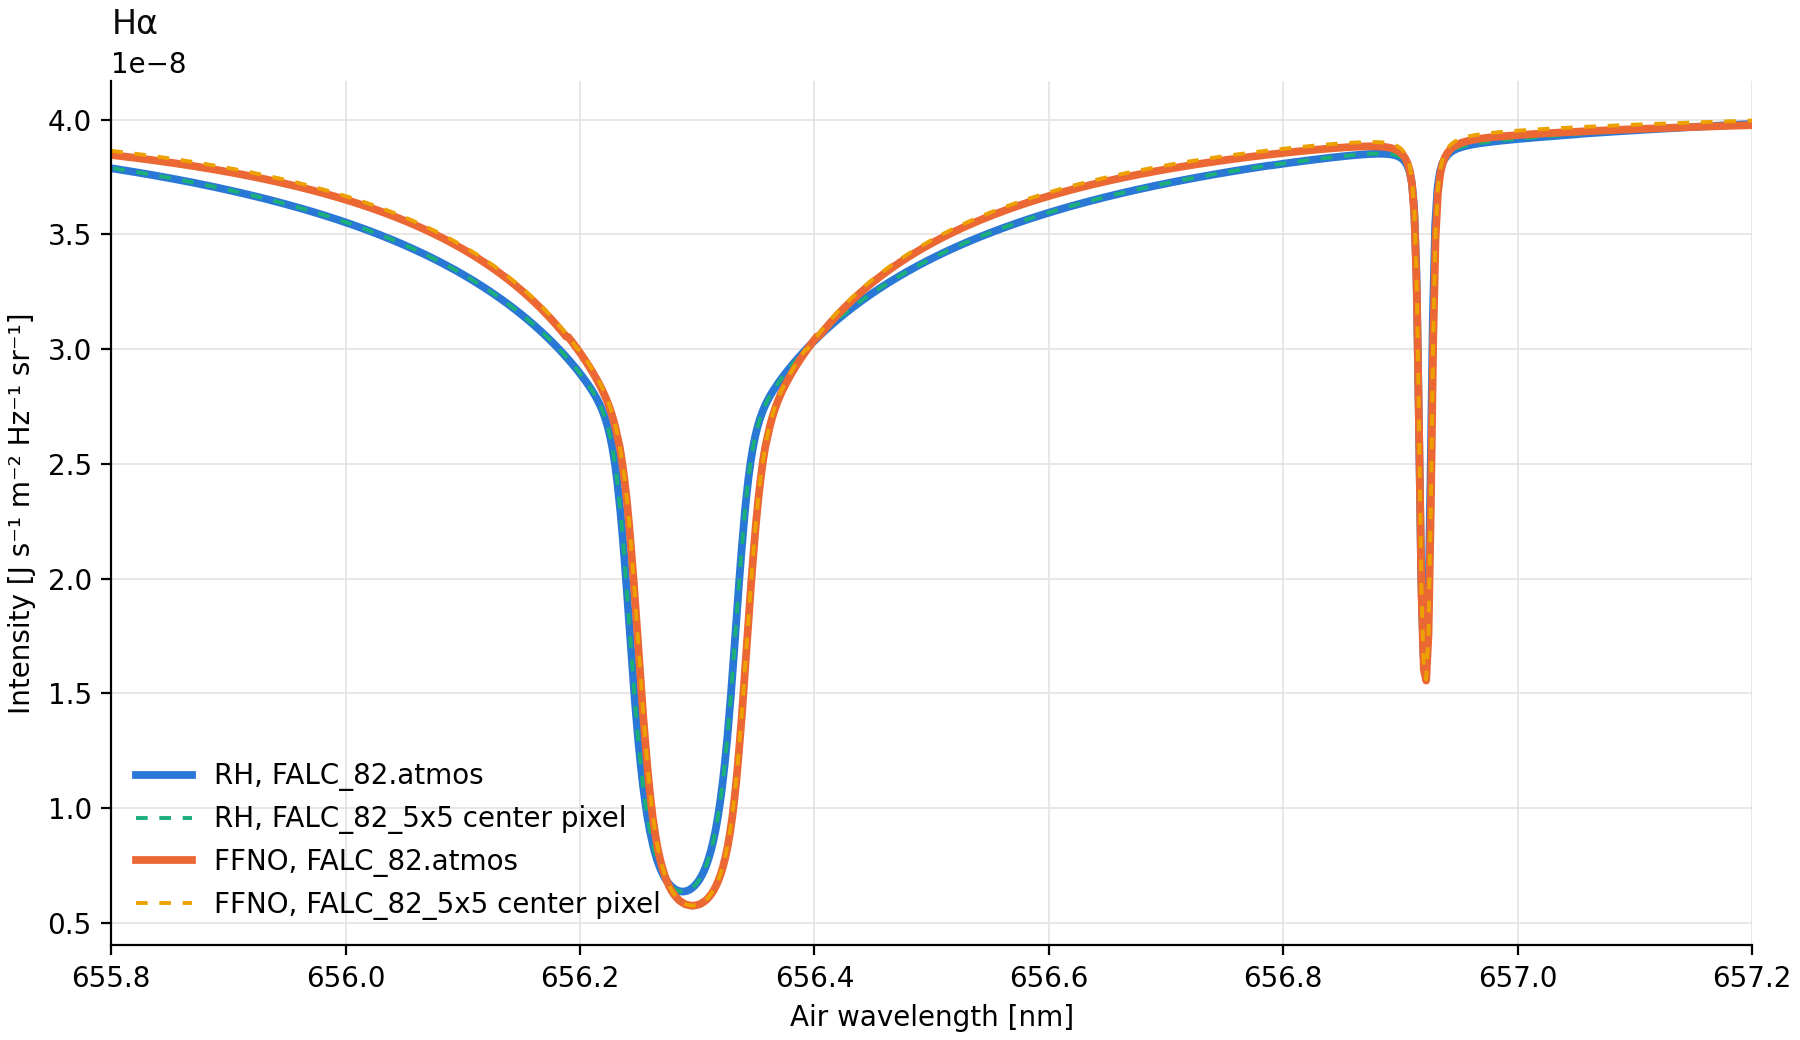
\includegraphics[width=.49\linewidth]{figures/falc_cmp_halpha.png}\hfill
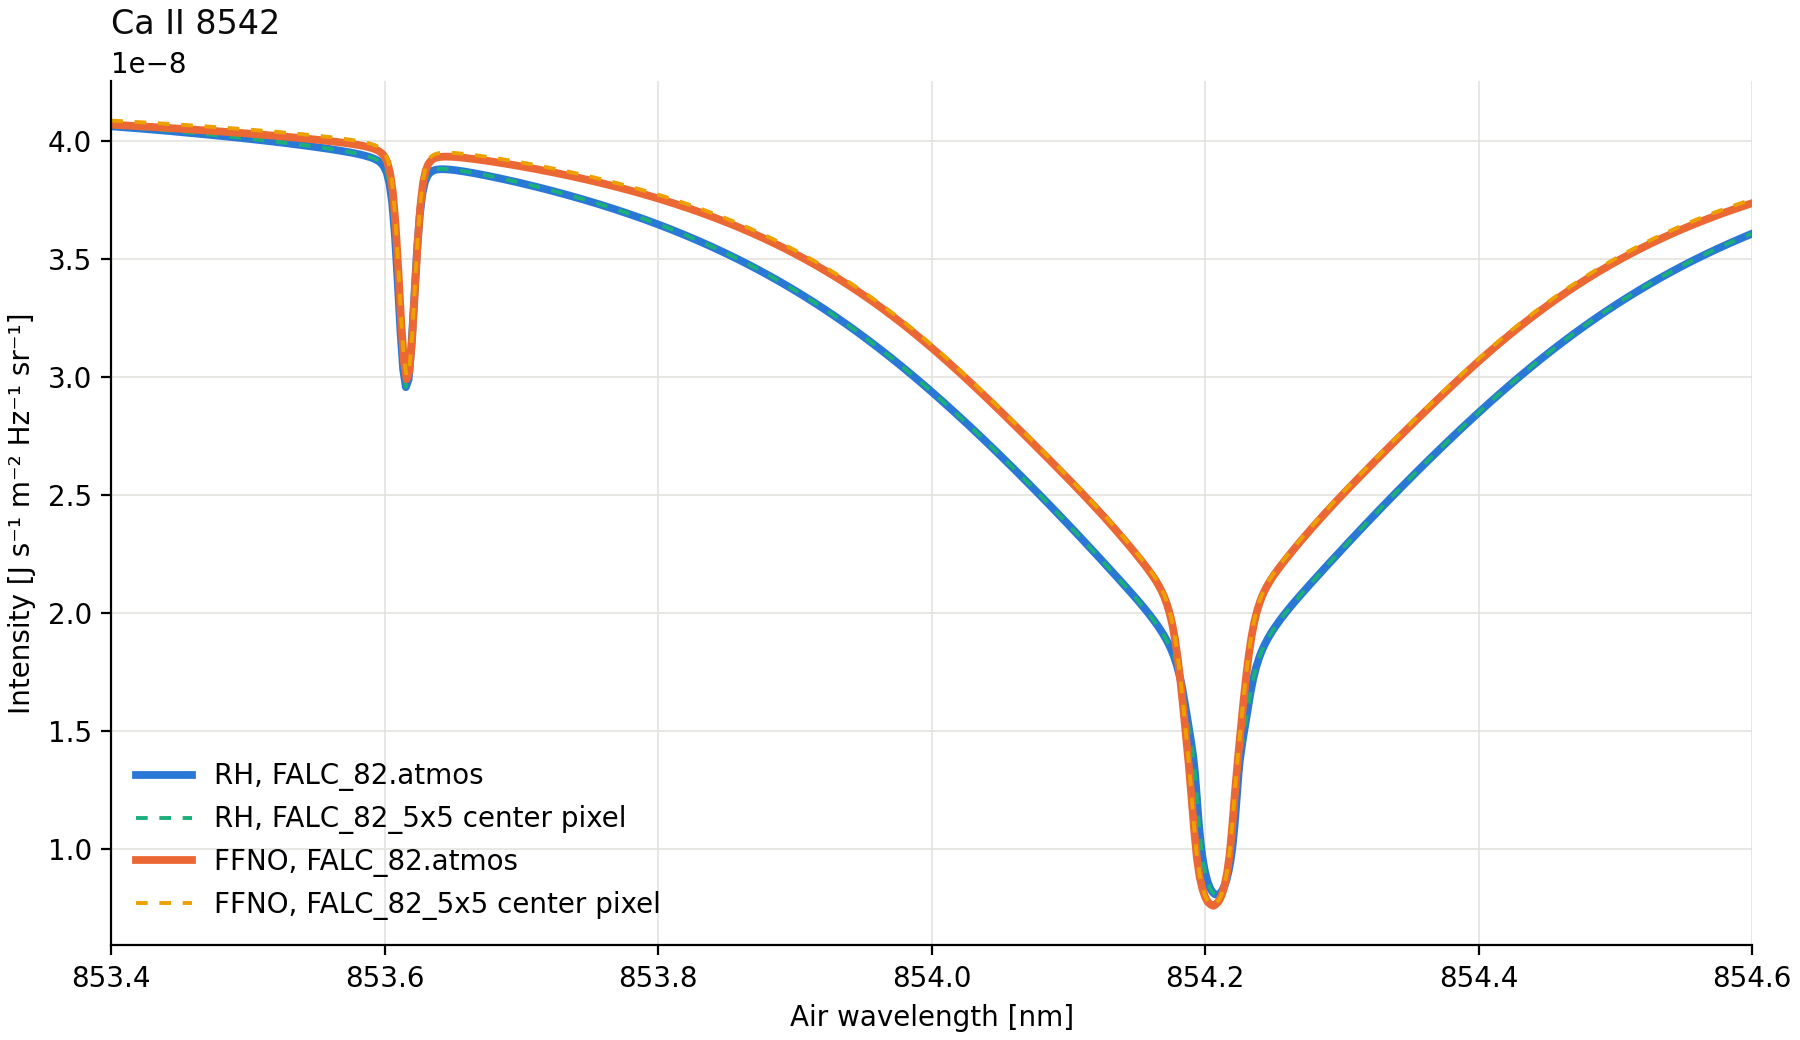
\includegraphics[width=.49\linewidth]{figures/falc_cmp_ca8542.png}
\caption{RH and FFNO on \code{FALC_82.atmos} and the centre pixel of \code{FALC_82_5x5.hdf5}, each with its own $\nel$ and hydrogen populations, using each code's unedited atoms and air wavelengths. The \Halpha{} cores differ by 0.08\,\AA{} (3.8\,km\,s$^{-1}$) because the atom files' level energies differ.}\label{fig:falc}
\end{figure}

A 1D model is far outside the training set, so Figure~\ref{fig:falc} is a stress test. The median difference from RH is about 2\% at \Halpha{} and 5\% at Ca\,\textsc{ii}, and FFNO's cores are about 10\% and 6\% deeper. RH treats H Ly$\alpha$, Ly$\beta$ and Ca\,\textsc{ii} H and K in PRD, which FFNO's training labels may treat differently; only the synthesis side of FFNO is known to be non-PRD. The two descriptions of the same model differ by 0.04\% in RH and about 1\% in FFNO.

\subsection{Where populations fail}
\begin{table}[H]\centering\small
\begin{tabularx}{\linewidth}{lYY}
\toprule
Cause&Where&Evidence\\\midrule
Column context&Sub-surface offsets of $-0.2$ to $-0.8$\,dex in the 16.8\,Mm tall boxes&Local inputs lie within the training distribution, but the column span does not. Cropping the column flips the sign.\\
Missing coverage&H corona above $\log T=6.05$&Training coverage is about zero.\\
Weak generalization&Cool, rarefied chromospheric gas in both species; time drift of \code{nw012023}&Coverage is normal, but held-out error is 3--4 times training error. The \code{nw012023} 1120 offset survives every crop.\\
Physics, unconfirmed&Helium simulation&$\nel$ at fixed $(T,\rho)$ scatters by $\pm0.3$\,dex against the other runs.\\\bottomrule
\end{tabularx}
\caption{Failure regimes from the uncertainty study (\code{docs/ffno3d-uq-report.md}). These are associations with partial experimental support, not proven causes.}
\end{table}

The dependence on column extent is strong: even training snapshot \code{nw012023} 915 shifts by 0.1--0.3\,dex under a moderate crop, and a hard crop to $z\le4$\,Mm gives errors of 0.5--0.9\,dex. So predictions should be trusted only for column extents seen in training.

\subsection{Horizontal boundaries}
The horizontal Fourier layers are periodic, as the simulations are, but the small $3\times3\times3$ convolution in the fusion step pads with zeros. This breaks horizontal translation invariance near the box edge. Repeating one real column over a square grid (H model, largest difference over depth and level) measured this directly:

\begin{table}[H]\centering\small
\begin{tabular}{lrrrrrrr}
\toprule
Distance from the edge [pixels]&0&1&2&3&4&6&9\\\midrule
Largest $|\Delta\log_{10}n|$ from the centre, $21\times21$ grid [dex]&0.492&0.099&0.052&0.026&0.017&0.006&0.001\\\bottomrule
\end{tabular}
\caption{Identical inputs give different outputs near the edge. The difference falls off inward, with a long tail because later Fourier layers carry it across the box. On a $5\times5$ grid the first ring from the edge differs from the centre by 0.14\,dex. This is the likely origin of the roughly 4\% spread between identical columns in the FAL-C spectra.}
\end{table}

For a periodic cube, this means the outer few columns of any prediction are affected by a boundary that does not physically exist.

\subsection{Is an uncertainty available?}
\begin{table}[H]\centering\small
\begin{tabularx}{\linewidth}{lY}
\toprule
Indicator&Measured behaviour\\\midrule
MC dropout&Spread is 6--25 times too small, and does not grow with distribution shift. Not usable for H.\\
Distance to training data&Weak for H (case rank correlation 0.40), good for Ca (0.71).\\
Conservation residual $|\log\sum n_i-\log n_{\rm element}|$&Free and needs no labels. Best H indicator (case rank correlation 0.55; its top 5 are among the 6 worst cases). Blind to errors within the total, such as a wrong Ca ionization balance.\\\bottomrule
\end{tabularx}
\caption{Candidate uncertainty indicators. There is no calibrated predictive uncertainty yet.}
\end{table}

\section{Assumptions and limits}
\begin{itemize}
\item \textbf{Statistical equilibrium in the labels.} The labels are MULTI3D's solution for the given snapshot. FFNO does not model time-dependent population evolution.
\item \textbf{Fixed atom, fixed lines.} Six-level H and Ca\,\textsc{ii} from these files. New atoms need new labels and training. Only \Halpha{} and Ca\,\textsc{ii} 854.2\,nm are synthesized from FFNO populations; other transitions are possible in principle but are not wired into the inversion code.
\item \textbf{Non-PRD, Stokes $I$.} Polarization and PRD are not implemented in synthesis.
\item \textbf{Hydrostatic columns} in the inversion. MHS modes exist in HSEMHS but are not connected, and the boundary pressure is not a control.
\item \textbf{LTE EOS} for $P$, $\rho$, $\nel$ and $\chi_{500}$, in a chromosphere that is not in LTE. Composition also differs slightly from the training simulations, whose $\rho/(n_{\rm H}m_{\rm H})$ is 1.357, against 1.398 for Wittmann's composition.
\item \textbf{Continuum in LTE form}, with hydrogen from the EOS, and scattering treated as thermal.
\item \textbf{Domain of validity.} Bifrost-like solar atmospheres on grids resembling the training grids, with column extents seen in training. No guard stops a user from going beyond this. Very hot corona, new magnetic regimes and other stars are unvalidated.
\item \textbf{Network derivatives} are used in the gradient but were never trained on.
\end{itemize}

\appendix
\section{Notation}
\begin{tabularx}{\linewidth}{>{$}l<{$}Yl}
\toprule
\text{Symbol}&Meaning&Unit\\\midrule
T,P,\rho&temperature, gas pressure, mass density&K, Pa, kg\,m$^{-3}$\\
\nel,\ n_{\rm H\,I},\ n_{\rm p}&electrons, neutral hydrogen, protons&m$^{-3}$\\
n_i,\ n_i^*,\ b_i&level population, LTE population, departure coefficient&m$^{-3}$, m$^{-3}$, --\\
\mathbf v,\ \vlos,\ \vturb&velocity, line-of-sight component ($\mathbf n\cdot\mathbf v$), microturbulence&m\,s$^{-1}$\\
z,\ m,\ \tau_{500}&height (upward), column mass, optical depth at 500\,nm&m, kg\,m$^{-2}$, --\\
\chi_\lambda,\ \eta_\lambda,\ S_\lambda&extinction, emissivity, source function&m$^{-1}$, --, --\\
\mu,\ \phi,\ \mathbf t&$\cos\theta$, azimuth from $+x$ toward $+y$, slant $\tan\theta(\cos\phi,\sin\phi)$&--\\
g&solar surface gravity, 274&m\,s$^{-2}$\\\bottomrule
\end{tabularx}

\section{Further reading}
\begin{itemize}
\item D.~Mihalas, \emph{Stellar Atmospheres} (1978); R.~J.~Rutten, \emph{Radiative Transfer in Stellar Atmospheres} (lecture notes): the NLTE theory of Sections 2--3.
\item J.~Leenaarts \& M.~Carlsson (2009), MULTI3D. B.~Gudiksen et al.\ (2011), Bifrost. The sources of the labels.
\item H.~Uitenbroek (2001), RH. T.~Pereira \& H.~Uitenbroek (2015), RH 1.5D. The reference codes in Section~\ref{sec:validation}.
\item Z.~Li et al.\ (2021), Fourier neural operators. A.~Tran et al.\ (2023), factorized FNOs. The operator-learning background.
\item J.~Fontenla, E.~Avrett \& R.~Loeser (1993), the FAL atmospheres.
\item In this repository: \code{FFNOInversion.jl/docs/viewing-angle/README.md}, \code{docs/ffno3d-uq-report.md}. In the HSEMHS repository: \code{docs/physics/}.
\end{itemize}
\end{document}
